\documentclass[tikz]{standalone}
\usepackage{amsmath}
\usetikzlibrary{arrows.meta,positioning,calc,fit}

\begin{document}
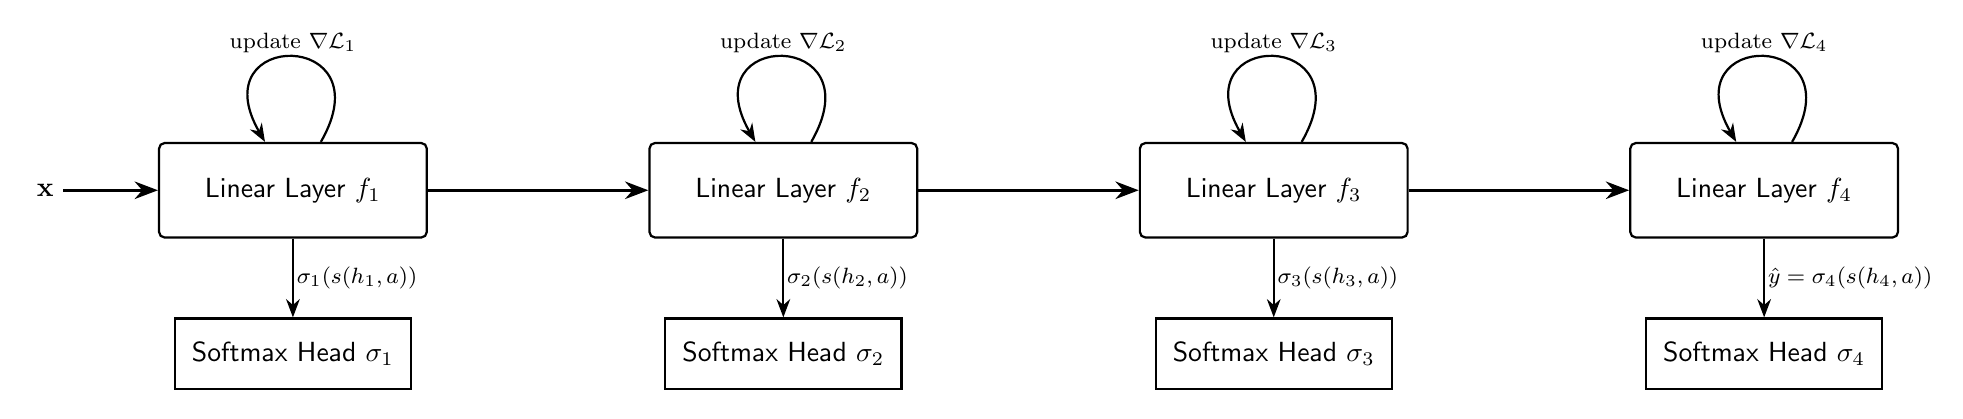
\begin{tikzpicture}[
  font=\sffamily,
  >=Stealth,
  node distance=22mm,
  block/.style={draw, rounded corners=2pt, minimum width=34mm, minimum height=12mm, align=center, thick, fill=white},
  head/.style={draw, minimum width=30mm, minimum height=9mm, align=center, thick, fill=white},
  arrow/.style={-Stealth, very thick},
  thinarrow/.style={-Stealth, thick},
  note/.style={font=\footnotesize, inner sep=1pt}
]

% ----- INPUT -----
\node (x) {$\mathbf{x}$};

% ----- LAYER BLOCKS -----
\node[block, right=12mm of x] (b1) {Linear Layer $f_1$};
\node[block, right=28mm of b1] (b2) {Linear Layer $f_2$};
\node[block, right=28mm of b2] (b3) {Linear Layer $f_3$};
\node[block, right=28mm of b3] (b4) {Linear Layer $f_4$};

% ----- HEADS (Similarity + Softmax) -----
\node[head, below=10mm of b1] (h1) {Softmax Head $\sigma_1$};
\node[head, below=10mm of b2] (h2) {Softmax Head $\sigma_2$};
\node[head, below=10mm of b3] (h3) {Softmax Head $\sigma_3$};
\node[head, below=10mm of b4] (h4) {Softmax Head $\sigma_4$};

% ----- SHARED LABEL ANCHORS (OPTIONAL VISUAL) -----
% (Shown once for clarity; all heads use the same anchors.)

% ----- FORWARD CONNECTIONS -----
\draw[arrow] (x) -- node[below, note]{} (b1);
\draw[arrow] (b1) -- node[below, note]{} (b2);
\draw[arrow] (b2) -- node[below, note]{} (b3);
\draw[arrow] (b3) -- node[below, note]{} (b4);



% ----- BRANCHES TO HEADS -----
\draw[thinarrow] (b1.south) -- node[right, note]{$\sigma_1(s(h_1, a))$} (h1.north);
\draw[thinarrow] (b2.south) -- node[right, note]{$\sigma_2(s(h_2, a))$} (h2.north);
\draw[thinarrow] (b3.south) -- node[right, note]{$\sigma_3(s(h_3, a))$} (h3.north);
\draw[thinarrow] (b4.south) -- node[right, note]{$\hat y = \sigma_4(s(h_4, a))$} (h4.north);

% ----- SELF-LOOPS (LOCAL LAYER-WISE GREEDY UPDATE) -----
% Self-loop using out/in with high looseness to create a loop over each block
\draw[thinarrow] (b1) to[out=60, in=120, looseness=6] node[above, note]{update $\nabla\mathcal{L}_1$} (b1);
\draw[thinarrow] (b2) to[out=60, in=120, looseness=6] node[above, note]{update $\nabla\mathcal{L}_2$} (b2);
\draw[thinarrow] (b3) to[out=60, in=120, looseness=6] node[above, note]{update $\nabla\mathcal{L}_3$} (b3);
\draw[thinarrow] (b4) to[out=60, in=120, looseness=6] node[above, note]{update $\nabla\mathcal{L}_4$} (b4);

% ----- OPTIONAL: OUTPUT NOTE -----
% \node[anchor=west, note] at ($(b4.east)+(16mm,0)$) {final layer used for inference};

\end{tikzpicture}
\end{document}